
\newpage
\setlength{\voffset}{-3cm}

\begin{center}
\section{\textbf{\huge{User Handling}}}

\Large{Use Cases}
\end{center}

%--------START EDITING HERE FOR HANDLING---------
%Maria %

%--------USER LOGIN---------
\subsection{User login}
\textbf{Description:}
This use-case enables a user to log into the system so as to insert medical data.
\subsubsection{Prioritization:}
Critical
\subsubsection{Conditions and Data Structures:}
\textbf{Pre-Conditions:}
\begin{itemize}
	\item , The user must be found on LDAP, thus have a valid username and password.
	\item The user must not already be logged in.
\end{itemize}

\textbf{Post-Conditions:}	
\begin{itemize}
	\item The user is loged in.
	\item The user is authenticated.
	\item The user can carry out system activities.
\end{itemize}
\subsubsection{Process Specifications:} 
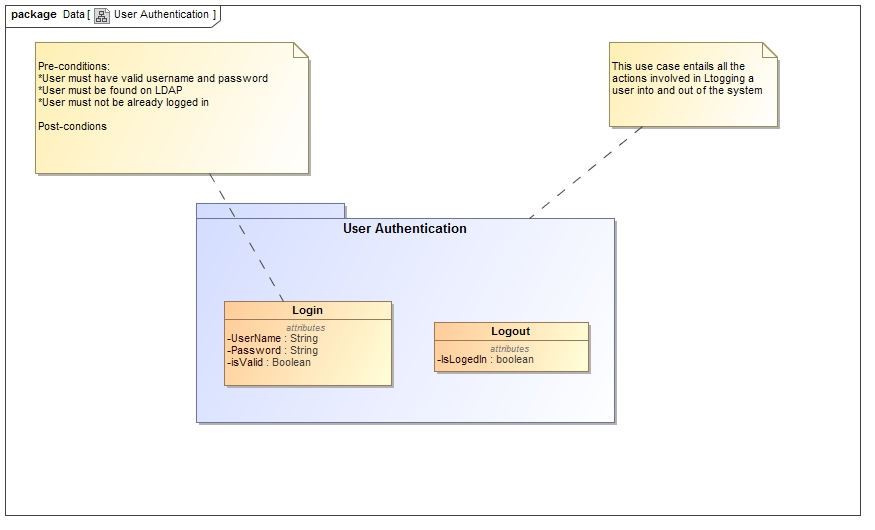
\includegraphics[width=1\linewidth]{./Graphics/Login}


%--------USER LOGOUT---------
\subsection{Logout}
\textbf{Description:}
User Is logged out of system and is not allowed to access system until logged in again
\subsubsection{Prioritization:}
Crucial
\subsubsection{Conditions and Data Structures:}
\textbf{Pre-Conditions:}
\begin{itemize}
	\item The user must be actively loged in
\end{itemize}
\textbf{Post-Conditions:}	
\begin{itemize}
	\item The user is logged out of the system
\end{itemize}
\subsubsection{Process Specifications:}
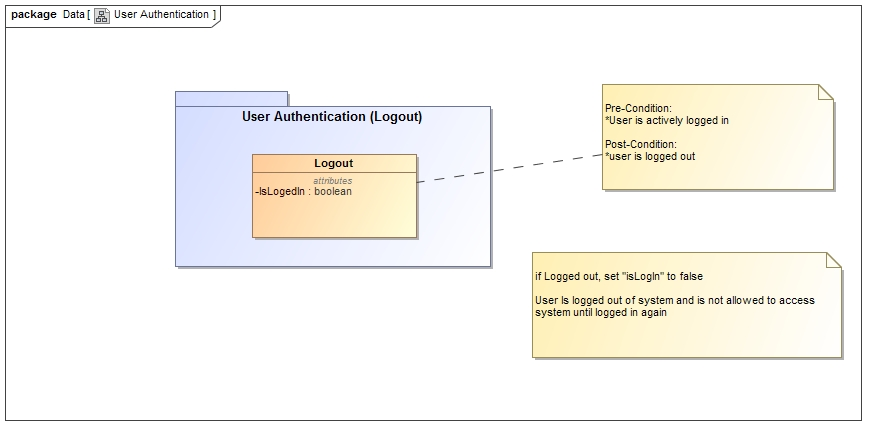
\includegraphics[width=1\linewidth]{./Graphics/Logout}

